\section{Marco teórico}

\subsection{Circuito resonante RLC}

Un circuito resonante está compuesto por una resistencia, bobina y un capacitor (Figura 1), en el cual se produce una resonancia en una frecuencia determinada. La frecuencia de resonancia es aquella en 
la cual la reactancia inductiva y la reactancia capacitiva son iguales, por lo que la impedancia del circuito es puramente resistiva. 

\begin{figure}[h]
    \centering
    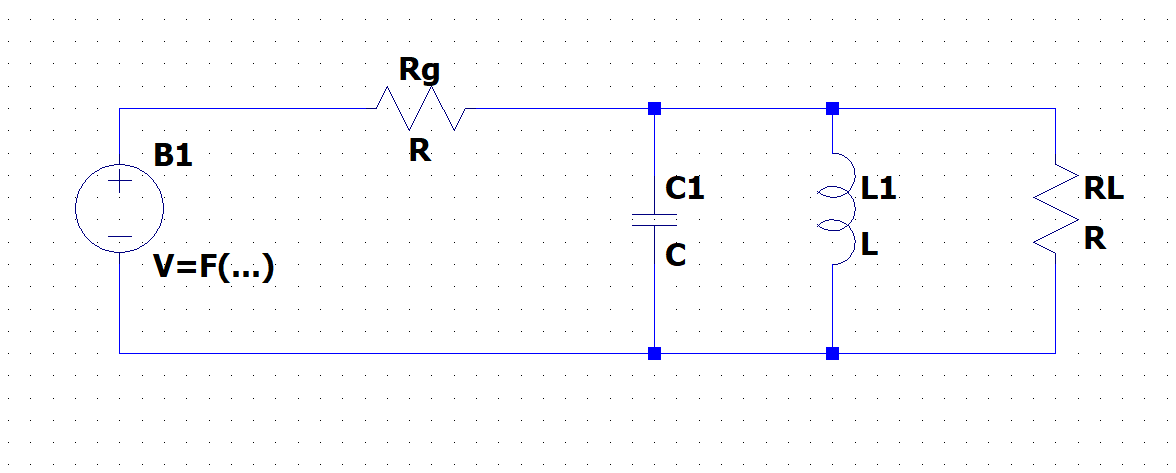
\includegraphics[width=0.5\textwidth]{Imagenes/circuito_resonante.png}
    \caption{Circuito resonante RLC}
    \label{fig:circuito_resonante}
\end{figure}

La frecuencia de resonancia o frecuencia central ($f_0$) caracteriza al circuito resonante, y se calcula mediante la siguiente ecuación:

\begin{equation}
    f_0 = \frac{1}{2\pi \sqrt{LC}}
\end{equation}

Donde: 
\begin{itemize}
    \item $f_0$ es la frecuencia central
    \item $L$ es la inductancia
    \item $C$ es la capacidad
\end{itemize}

En la última ecuación podemos observar que la frecuencia central depende de la inductancia $L$ y la capacidad $C$. 
A partir de la $f_0$ podemos definir el factor de calidad cuando el circuito está cargado ($Q_c$) y cuando el circuito está descargado ($Q_d$). 
Se pueden calcular mediante las siguientes ecuaciones:

\begin{equation}
    Q_c = \frac{f_0}{BW} = \frac{R_T}{X_L}
\end{equation}

\begin{equation}
    Q_d = \frac{R_P}{X_L}
\end{equation}

Donde: 

\begin{itemize}
    \item $R_T$ es la resistencia total
    \item $R_P$ es la resistencia paralelo
    \item $X_L$ es la reactancia inductiva
    \item $BW$ es el ancho de banda
\end{itemize}

La variable $R_T$ es la resistencia total del circuito, la cual determinará el factor de calidad cargado del circuito. 
El inductor real tendrá pérdidas parasitarias, esta resistencia se encuentra en paralelo con el inductor
de la figura 1 y se denomina resistencia en paralelo ($R_P$). La resistencia total del circuito $R_T$ se calcula mediante la siguiente ecuación:

\begin{equation}
    R_T = R_P \parallel R_L \parallel R_g
\end{equation}

Donde:
\begin{itemize}
    \item $R_P$ es la resistencia paralelo
    \item $R_L$ es la resistencia de carga
    \item $R_g$ es la resistencia del generador
\end{itemize}

En este trabajo práctico se pretende diseñar un circuito resonante a una determinada frecuencia central y ancho de banda. Por lo tanto realizaremos una 
modificación del circuito de la figura 1, para obtener el circuito de acoplamiento interetapas (Figura 2). 

\begin{figure}[h]
    \centering
    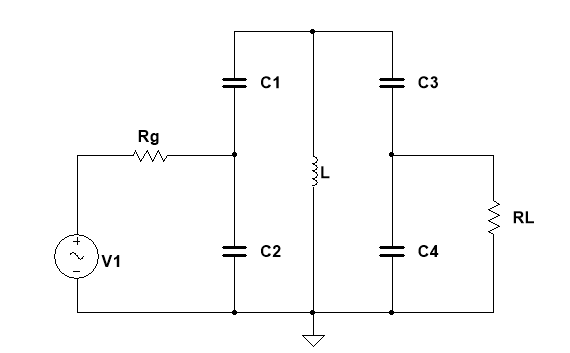
\includegraphics[width=0.5\textwidth]{Imagenes/circuito_acoplamiento2.png}
    \caption{Circuito de acoplamiento interetapas RLC modificado}
\end{figure}

El circuito de la figura 2 tiene la misma frecuencia central que el circuito de la figura 1. Si calculamos la capacidad total, obtendremos la misma que la del circuito de la figura 1.

\begin{equation}
    C_T = \frac{C1 \cdot C2}{C1 + C2} + \frac{C3 \cdot C4}{C3 + C4} = \frac{C}{2} + \frac{C}{2} 
\end{equation}

Analizando la salida del circuito de la figura 2, podemos trazar un paralelismo con el autotransformador, donde podemos reflejar las impedancias tanto del 
generador como de la carga al primario. Y donde cada capacitor o la suma de ellos es el bobinado del autotransformador.

\begin{figure}[h]
    \centering
    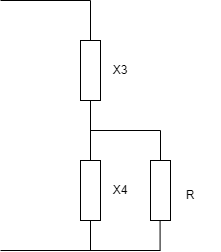
\includegraphics[width=0.3\textwidth]{Imagenes/Esquema_autotrafo.png}
    \caption{Autotransformador}
\end{figure}

Del autotransformador podemos obtener la relación de transformación:

\begin{figure}[h]
    \centering
    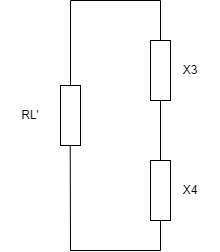
\includegraphics[width=0.3\textwidth]{Imagenes/relacion_transformacion.png}
    \caption{Esquema de relación de transformación}
\end{figure}

\begin{equation}
    R_L' = (1 + \frac{C_3}{C_4})^2 \cdot R_L 
\end{equation}

\begin{equation}
    R_g' = (1 + \frac{C_1}{C_2})^2 \cdot R_g
\end{equation}

Finalmente, el circuito reflejado de la figura 2 queda como se muestra en la figura 5:

\begin{figure}[h]
    \centering
    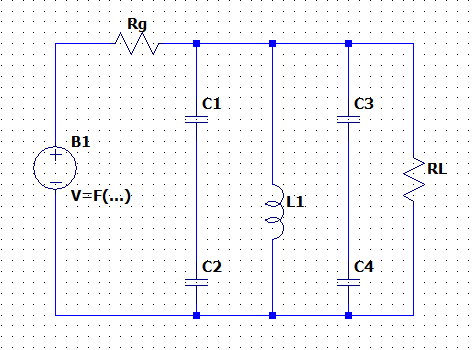
\includegraphics[width=0.5\textwidth]{Imagenes/circuito_reflejado.png}
    \caption{Circuito reflejado}
\end{figure}

Donde nos queda una resistencia total de:

\begin{equation}
    R_T = R_g' \parallel R_L' \parallel R_P
\end{equation}

Donde:

\begin{itemize}
    \item $R_g'$ es la resistencia del generador reflejada
    \item $R_L'$ es la resistencia de carga reflejada
    \item $R_P$ es la resistencia paralelo
\end{itemize}

Con el circuito reflejado, las resistencias $R_g'$ y $R_L'$ dependerán de los capacitores $C1$, $C2$, $C3$ y $C4$, lo que nos permitirá adaptar las impedancias de entrada y salida del circuito.
Podemos realizar la siguiente asignación de valores, donde seguiremos cumpliendo la condición de la ecuación 7:

\begin{equation}
    R_T = X_L \cdot Q_c = R_g' \parallel (R_L' \parallel R_P) = 2 R_T \parallel 2 R_T 
\end{equation}

Finalmente, luego de este desarrollo nos quedará un sistema de ecuaciones con 4 incógnitas, las cuales son $C1$, $C2$, $C3$ y $C4$, que nos servirán para el diseño del circuito de acoplamiento.

\begin{equation}
    \begin{cases}
        R_L' = \left(1 + \frac{C_3}{C_4}\right)^2 \cdot R_L \vphantom{\frac{C_1 \cdot C_2}{C_1 + C_2}} \\
        \\
        R_g' = \left(1 + \frac{C_1}{C_2}\right)^2 \cdot R_g \vphantom{\frac{C_1 \cdot C_2}{C_1 + C_2}} \\
        \\
        \frac{C_1 \cdot C_2}{C_1 + C_2} = \frac{C}{2} \\
        \\
        \frac{C_3 \cdot C_4}{C_3 + C_4} = \frac{C}{2}
    \end{cases}
\end{equation}

\subsection{Condición para la reflexión de impedancias}

La demostración de la reflexión de impedancias se parte de un circuito mixto y se lo lleva a otro paralelo. En la siguiente figura se muestran la forma que queremos expresar el circuito.

\begin{figure}[h]
    \centering
    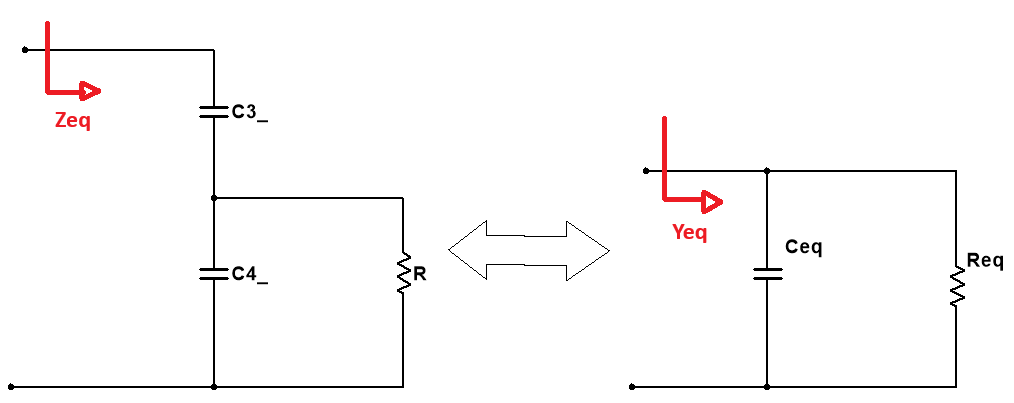
\includegraphics[width=0.8\textwidth]{Imagenes/reflexion_impedancias.png}
    \caption{Circuitos equivalentes}
\end{figure}

La impedancia equivalente del circuito mixto se puede expresar como:

\begin{equation}
    Z_{eq} = X_{C3} + X_{C4} // R 
\end{equation}

Desarrollando la ecuación anterior, obtenemos:

\begin{equation}
    Z_{eq} = \frac{R \cdot (1 + \frac{C4}{C3}) - j \cdot \frac{1}{2 \pi f C3}}{1 + j \cdot R \cdot 2 \pi f C4} 
\end{equation}

Luego para pasar al modelo equivalente paralelo podremos expresar la impedancia como admitancia para mayor facilidad de cálculo:

\begin{equation}
    Y_{eq} = \frac{1}{Z_{eq}} = \frac{1 + j \cdot R \cdot 2 \pi f C4}{R \cdot (1 + \frac{C4}{C3}) - j \cdot \frac{1}{2 \pi f C3}}
\end{equation}

Racionalizando la expresión:

\begin{equation}
    Y_{eq} =  \frac{1}{Z_{eq}} = \frac{1 + j \cdot R \cdot 2 \pi f C4}{R \cdot (1 + \frac{C4}{C3}) - j \cdot \frac{1}{2 \pi f C3}} \cdot \frac{R \cdot (1 + \frac{C4}{C3}) + j \cdot \frac{1}{2 \pi f C3}}{R \cdot (1 + \frac{C4}{C3}) + j \cdot \frac{1}{2 \pi f C3}}
\end{equation}

Finalmente, obtenemos la expresión de la admitancia equivalente:

\begin{equation}
    Y_{eq} = \frac{R + j \cdot (2 \pi)^2 \cdot f^2 \cdot C4 \cdot (1 + \frac{C4}{C3})}{R^2 \cdot (1 + \frac{C4}{C3})^2 + \frac{1}{4 \pi^2 f^2 C3^2}}
\end{equation}

Tomando la parte real de la admitancia para obtener la conductancia equivalente:

\begin{equation}
    G_{eq}= Re(Y_{eq}) = \frac{R}{R^2 \cdot (1 + \frac{C4}{C3})^2 + \frac{1}{4 \pi^2 f^2 C3^2}}
\end{equation}

Simplificando e invirtiendo la expresión, obtenemos la $R_{eq}$ que es la resistencia equivalente del circuito paralelo que inicialmente queremos:

\begin{equation}
    R_{eq} = R \cdot (1 + \frac{C4}{C3})^2 + \frac{1}{R \cdot 4 \pi^2 f^2 C3^2}
\end{equation}

El segundo término de la ecuación 17 hace que no se cumpla la reflexión de impedancias. Para solucionar este problema, se debe cumplir la siguiente condición:

\begin{equation}
    R \cdot 4 \pi^2 f^2 C3^2 \gg 10 
\end{equation}

El parámetro que podremos variar para cumplir la condición de la ecuación 18 es la capacidad de C3. 
